%TEX root = ./overwiew.tex

\documentclass{standalone}

\usepackage{tikz}
\usetikzlibrary{positioning}
\usetikzlibrary{shapes,arrows}


\begin{document}
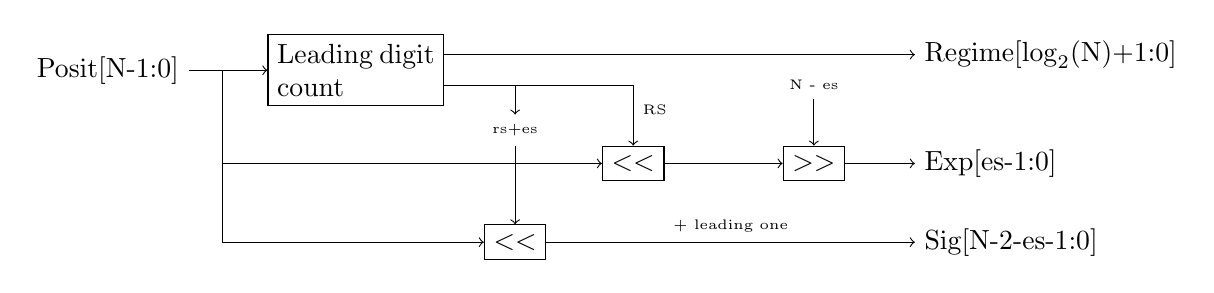
\begin{tikzpicture}
	\node (lc) {};
	\node (rc) [below right =2cm and 10cm of lc] {};

	\node (posit) [left, below=0cm of lc] {Posit[N-1:0]};
	\node (pl) [below right=-0.55cm and 0.3cm of posit] {};
	\node[draw] (ldc) [right=1cm of posit] {\parbox{2cm}{Leading digit count}};
	\node[draw] (lshift) [below right=0.5cm and 2cm of ldc] {$<<$};
	\node[draw] (rshift) [right=1.5cm of lshift] {$>>$};
	\node (shval) [above of= rshift] {\tiny N - es};
	\node[draw] (lsh) [below right=1.5cm and 0.5cm of ldc] {$<<$};
	\node (esplus) [above=1cm of lsh] {\tiny rs+es};
	% \node[draw] (esh2) [right of= esh1] {$>>$};
	% \node[draw] (fsh) [below right=0.5cm and 1cm of esh2] {$>>$};



	\path [draw, ->] (posit) -- (ldc);
	\path [draw, ->] (ldc.10) -- (ldc.10 -| rc) node [right] {Regime[$\log_2$(N)+1:0]};
	\path [draw, ->] (ldc.-10) -| (lshift) node[above right=0.5cm and 0cm] {\tiny RS};
	\path [draw, ->] (pl) |- (lshift);
	\path [draw, ->] (lshift) -- (rshift);
	\path [draw, ->] (shval) -- (rshift);
	\path [draw, ->] (rshift) -- (rshift -| rc) node [right] {Exp[es-1:0]};
	\path [draw, ->] (pl) |- (lsh);
	\path [draw, ->] (ldc.-10) -| (esplus);
	\path [draw, ->] (esplus) -- (lsh);
	\path [draw, ->] (lsh) -- node [above, midway] {\tiny + leading one} (rc |- lsh) node [right] {Sig[N-2-es-1:0]};
\end{tikzpicture}
\end{document}